\chapter{Perancangan}
\label{chap:Perancangan}

Pada bab ini dijelaskan mengenai perancangan perangkat lunak yang dibangun, meliputi perancangan kelas dan perancangan antarmuka.

\section{Perancangan Kelas}
\label{sec:perancangan_kelas}
\begin{figure}[H]
	\centering
		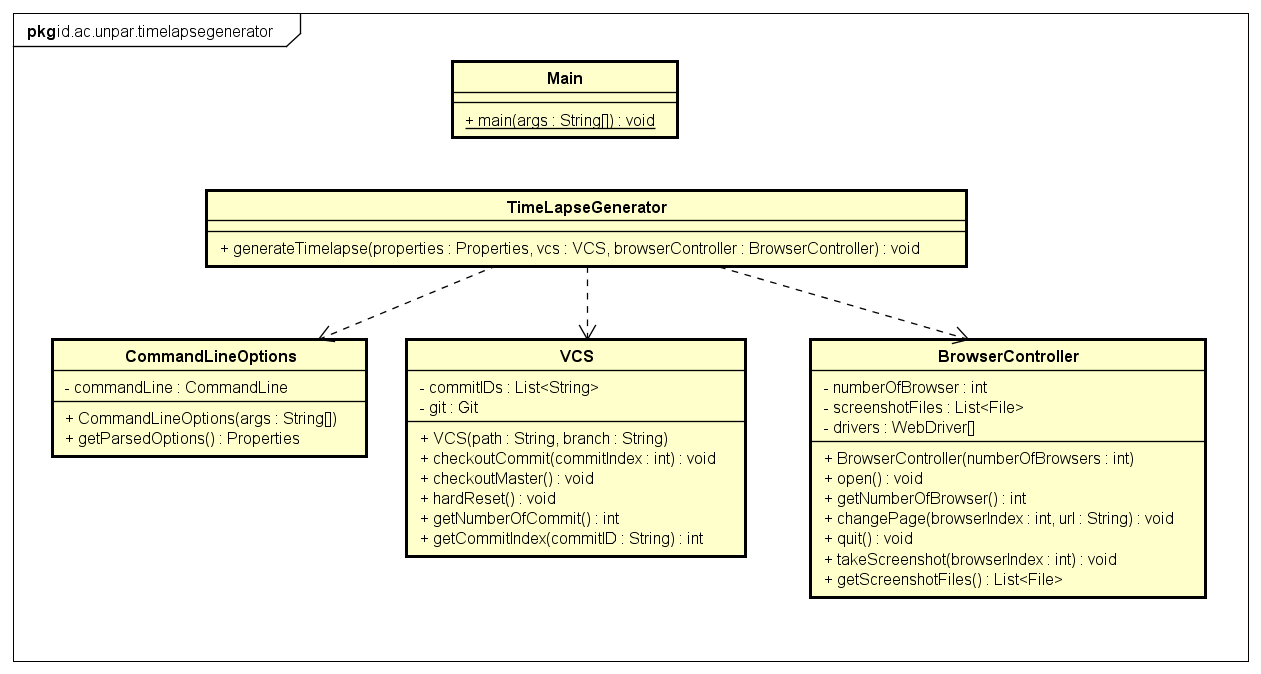
\includegraphics[scale=0.5]{Gambar/ClassDiagram.png}
	\caption{Diagram kelas.}
	\label{fig:class_diagram}
\end{figure}

Program pada skripsi ini memiliki lima kelas. Diagram kelas pada program ini dapat dilihat pada Gambar \ref{fig:class_diagram}. Berikut adalah rincian kelas yang terdapat pada program ini:
\begin{itemize}
\item BrowserController\\
Kelas ini digunakan untuk mengatur \textit{browser}. Operasi-operasi yang dilakukan terhadap \textit{browser} yaitu membuka \textit{browser}, mengambil \textit{screenshot}, membuat \textit{browser window} menjadi maksimal, dan menutup \textit{browser}. Berikut adalah atribut yang terdapat pada kelas ini:
\begin{itemize}
   \item private final WebDriver[] drivers\\
   Atribut ini adalah kumpulan \textit{browser} yang digunakan untuk keperluan \textit{automation testing}. 
    \item private final List<File> screenshotFiles\\
	Atribut ini berfungsi untuk menyimpan \textit{file} hasil \textit{screenshot}.
	\item  private final int numberOfBrowser\\
	Atribut ini menyatakan jumlah \textit{browser} yang dimiliki oleh kelas ini. Jumlah maksimal dari \textit{browser} adalah empat.
\end{itemize}

Berikut adalah \textit{method} yang terdapat pada kelas ini:
\begin{itemize}
\item public BrowserController(int numberOfBrowsers)\\
Constructor dari kelas ini. Berfungsi untuk menginisialisasi atribut yang dimiliki oleh kelas ini. Parameternya adalah jumlah \textit{browser} yang dapat dimiliki oleh kelas ini.
  \item public void open()\\
  Berfungsi untuk membuka semua \textit{browser}, kemudian mengatur ukuran \textit{browser window} menjadi maksimal. 
  \item public int getNumberOfBrowser()\\
  Berfungsi untuk mengembalikan jumlah browser yang dimiliki kelas ini.
  \item public void changePage(int browserIndex, String url)\\
  Berfungsi untuk berpindah halaman pada \textit{browser} tertentu. Parameternya adalah alamat URL untuk berpindah halaman dan indeks \textit{browser} yang akan diubah halamannya.
  \item public void quit()\\
  Berfungsi untuk menutup semua \textit{browser}.
  \item public void takeScreenshot(int browserIndex)\\
  Berfungsi untuk mengambil \textit{screenshot} pada \textit{browser} tertentu dan menyimpannya ke atribut screenshotFiles. Parameternya adalah indeks \textit{browser} yang akan diambil screenshotnya.
\end{itemize}

\item CommandLineOptions\\
Kelas ini berfungsi untuk menyimpan semua Option yang terdapat dalam program ini, dan melakukan \textit{parsing} argumen Command Line Options yang dimasukkan oleh \textit{user}.  

Berikut adalah atribut yang terdapat pada kelas ini:
\begin{itemize}
    \item private final CommandLine commandLine\\
    Atribut ini berfungsi untuk melakukan \textit{parsing} argumen Command Line Options dan menampung hasilnya. 
\end{itemize}
Berikut adalah \textit{method} yang terdapat pada kelas ini:
\begin{itemize}
\item public CommandLineOptions(String[] args)\\
Merupakan Constructor dari kelas ini. Berfungsi untuk menentukan Option yang terdapat pada program dan melakukan parsing argumen Command Line. Parameternya adalah argumen Command Line Option yang didapatkan dari
kelas Main.
\item public Properties getParsedOptions()\\
Berfungsi untuk mengembalikan Command Line Option yang sudah diparsing.
\end{itemize}

\item VCS\\
Kelas ini digunakan untuk berinteraksi pada proyek perangkat lunak yang terekam oleh Git. Berikut adalah atribut yang terdapat pada kelas ini:
\begin{itemize}
   \item  private final Git git\\
   Atribut ini digunakan untuk melakukan interaksi pada proyek perangkat lunak yang terekam oleh Git.
   \item private final List<String> commitIDs\\
   Atribut ini digunakan untuk menampung seluruh \textit{commit} ID dari hasil penelusuran histori.   
\end{itemize}

Berikut ini adalah \textit{method} yang terdapat dalam kelas ini:
\begin{itemize}
\item public VCS(String path)\\
Constructor dari kelas ini. Berfungsi untuk menginisialisasi variabel git dan mendapatkan seluruh histori commit pada proyek perangkat lunak berbasis web. Parameternya adalah \textit{path} dari proyek perangkat lunak berbasis web.
\item public void checkoutCommit(int commitIndex)\\
Berfungsi untuk melakukan \textit{checkout} ke \textit{commit} tertentu. Parameter dari \textit{method} ini adalah indeks dari variabel commitIDs.
\item public void checkoutMaster()\\
Berfungsi untuk melakukan \textit{checkout} ke \textit{commit} terakir.
\item public void hardReset()\\
Berfungsi untuk melakukan operasi Git Reset. Operasi ini menghapus perubahan pada \textit{working tree} di \textit{commit} tertentu. 
\item public int getNumberOfCommit()\\
Berfungi untuk mendapatkan jumlah \textit{commit}.
\item public int getCommitIndex(String commitID)\\
Berfungsi untuk mendapatkan indeks dari variabel commitIDs. Parameternya adalah \textit{Commit} ID yang akan dicari indeksnya.
\end{itemize}


\item TimeLapseGenerator\\
Kelas ini digunakan untuk membangkitkan animasi \textit{timelapse}.
Berikut adalah \textit{method} yang dimiliki oleh kelas ini:
\begin{itemize}
\item public void generateTimelapse(Properties properties, VCS vcs, BrowserController browserController)\\
Berfungsi untuk membangkitkan animasi \textit{timelapse} berdasarkan langkah-langkah pada Bab \ref{subsec:langkah_animasi}. Hasil animasi berupa \textit{file} bertipe GIF. Parameternya adalah objek yang bertipe VCS, BrowserController, dan Properties. Parameter properties menampung key dan value dari Option yang sudah diparsing. 
\end{itemize}

\end{itemize}

\section{Perancangan Antarmuka}
\label{sec:perancangan_antarmuka}
